\chapter{Background}
\label{sec:background}

% Initially part of a rough draft of a paper I was writing. This section is mostly about automated weather radar image analysis
One area of computational research into the meteorological nature of weather radar scans is in the field of meteorological object tracking. 
The goal of this field is to identify “storm cells,” areas of localized convective activity, track their history in terms of evolution, merging, and splitting, and make short term forecasts about where they are going. 
The definition of the storm cells themselves is a matter of some debate, though some basic definitions exist from the perspective of remote sensing, such as that of \cite{lakshmanan2010objective}, who defines the cells as comprised of a 30 dbz horizontal reflectivity across a spatial area of 20 km$^2$. 
This area of research is not directly related to the object of this study, which is to correctly label scans as containing stratiform or convective activity, though it is related, and could be easily applied to this classification problem with minimal extra algorithmic overhead.

There are several approaches to this problem that have been explored in using algorithms to perform these objectives. 
Thunderstorm Identification, Tracking, Analysis, and Nowcasting (TITAN) \cite{dixon1993titan}, is an early algorithm designed to perform a similar task on NWS NEXRAD data. 
Another heuristic method, this system utilizes an empirically-determined horizontal reflectivity threshold, $T_z$, to locate spatially contiguous runs of high intensity returns within this single bin to designate as storm centroids. 
The Storm Cell Identification and Tracking (SCIT) algorithm \cite{johnson1998storm}, seeks to improve upon TITAN’s approach mainly by adding more reflectivity bins with which to organize storm decisions. 
The algorithm attempts to locate storm cell centroids in NWS NEXRAD radar data, and follow them in space and time. 
This method operates on a radial-by-radial basis, binning reflectivity values, and then checking for spatial proximity of the binned regions, assigning storm cell centroid status to those spatially proximate areas of high reflectivity. 
As \cite{lakshmanan2009efficient} points out, these two methods are limited by their requirement that spatially adjacent pixels must contain horizontal reflectivity values within certain thresholds to be considered by the algorithm as components for storm cell centroid candidates. 
That work describes a method that attempts to find storm cells via usage of the watershed transform, a technique pulled from the field of image processing, with a few tweaks to ensure that it performs well with weather radar imagery. 
Namely, they propose altering the “saliency” and “hysteresis” levels to allow the watershed to identify mature and growing storm cells while weeding out false positives. 
This approach negates the need for empirically-chosen global thresholds for bins, as it considers all possible thresholds when classifying the image. 
However, the method requires significant data preprocessing prior to its application, including filters to remove high frequency image content and quantization of values, which may remove useful local features from the image.

\section{Neural Networks}
\label{sec:background_neuralnetworks}
% This may be too much detail but I think it would be relevant to set up nomenclature and discuss neural network basics in this section
% I expect some of the people reading this will be unfamiliar with terminology, and it feels necessary for the sake of completeness.
% There are some papers worth citing that should be cited here, maybe an open source book?
% Neurons, Gradients, Forward Propagation, Backward Propagation, Linear Regression, Outputs (sigmoid and softmax)
% Cartoon of densely connected neurons in a small network
%
% My current plan is to start with a basic treatment of NNs in the Classifying chapter, with math there, to set the table for the reader in the sections that follow.
% This section should be more like a history lesson, bringing in some of the more major efforts. Discussing all kinds of examples of problems solved by machine learning, identifying gaps where this work hopes to fill.

\section{Image Classification with Machine Learning}
\label{sec:background_imageclassification}

% Discussion on Image classification in the broader field of image data machine learning, so that these terms can be used later in the document
Image Classification is a sub-field of a larger umbrella of image data machine learning that also includes image segmentation and semantic understanding. It is, however, the first step to achieving these latter two. Image Segmentation refers to...

% Discuss here some of the most well known papers and concepts around classifying image data. Things like Dropout, ReLU, Dense, BatchNormalization, Exploding and Vanishing Gradients,

\section{Transfer Learning}
\label{sec:background_transferlearning}

Transfer Learning is most often used to learn target tasks that differ from source tasks but reside in the same natural image domain. However, these architectures have been used to classify and segment image data
There have been a few efforts to apply deep learning algorithms in the area of climate science, applying models to weather data. 
For example, \cite{liu2016application} applied a deep learning architecture called AlexNet \cite{krizhevsky2012imagenet} to locate tropical cyclones, weather fronts, and atmospheric rivers, in colormapped continuous spatial variables, like precipitation, temperature, and other meteorological properties.
They briefly describe issues surrounding the usage machine learning models developed for natural image data in a non-natural-image data domain, and focus their analysis on a continental data scale.


\section{Dual-Polarized Doppler Weather Radar}
\label{sec:background_dualpol}
% This section is somewhat boilerplate in our group, but the basics of weather radar should be discussed here so that the instrument producing the data used in this research is understood. 
% Maybe a page or two, some images?

One of the key benefits \cite{doviak2000considerations} in dual-polarimetric Doppler weather radar over its predecessor, single-polarization, is that allows observing not only power return from a volume of scatterers, but also identifying parameters related to shape.
This is due to its usage of not only one antenna polarization in transmit and receive modes, but two orthogonally polarized antennas, which convey both power return in the horizontal as well as vertical.
For low elevation scans, as in those employed in plan-position indicator (PPI) scans, which are the focus of this research, these shape parameters can convey a great deal more information for the radar engineer to use in analysis.
This information is used directly by radar meteorologists to determine relevant atmospheric parameters with respect to various weather phenomena, as well as to inform several types of algorithms concerned with extracting additional information from these scans.
It is relevant to survey some of these techniques briefly here as many of the phenomena described tie directly into precipitation regime, and the methods utilized to extract key information as below directly inspires and influences the research presented in this work.
Some efforts of note along with brief descriptions:

\begin{itemize}
	\item Hydrometeor classification - determination of scatterer type in radar scans
	\begin{itemize}
		\item Using dual-polarizaton data to identify winter precipitation \cite{thompson2014dual}
		\begin{itemize}
			\item Using data from multiple radars and radar frequencies, this work uses scattering theory and T-matrix simulations to develop an algorithm based on fuzzy logic to classify scatterers in radar gates by their predominant hydrometeor type.
		\end{itemize}
		\item Semisupervised scheme for hydrometeor classification \cite{bechini2015semisupervised}
		\begin{itemize}
			\item Uses a fuzzy logic method as above, but adds a k-means clustering component to take advantage of localized spatial similarity of precipitation type to improve classification in range-height indicator (RHI) scans
		\end{itemize}
	\end{itemize}
	\item Nowcasting and short-term forecasting
	\begin{itemize} 
		\item LSTM model for precipitation nowcasting \cite{xingjian2015convolutional}
		\begin{itemize}
			\item Utilizes a memory-based neural network architecture called long short-term memory (LSTM) with a novel addition of convolutional input layers to utilize spatial and temporal information in short-term rainfall intensity prediction 
		\end{itemize}
		\item TITAN \cite{dixon1993titan}
		\begin{itemize}
			\item Early and well-known set of algorithms for identifying and tracking thunderstorms using NEXRAD WSR-88D data, using many image processing techniques with thresholded spatial and temporal information
		\end{itemize}
	\end{itemize}
	\item Quantitative precipitation estimation (QPE) - counting how much precipitation has already occurred 
	\begin{itemize}
		\item QPE in the CASA DFW Urban Testbed network \cite{chen2015quantitative}
		\begin{itemize}
			\item This paper computes the real-time rainfall rate in high spatio-temporal resolution by using information available from multiple radars scanning similar areas, on different time scales
		\end{itemize}
	\end{itemize}
\end{itemize}

This section intends to acquaint the reader with some of the major derived radar variables, with a focus on those that are used in this effort to classify stratiform and convective precipitation regimes both from one another and from cases that represent neither.
For a full treatment of weather radar theory, with specific focus on signal processing, consult \cite{bringi2001polarimetric} and \cite{doviak2006doppler}.


\subsection{Moments}
\label{ssec:background_moments}
% Moments refer to the different radar variables. 
% Talk about the big ones: reflectivity, differential reflectivity, copolar correlation, velocity, spectrum width, specific differential phase
% 

There are a few important radar variables, also called moments, that are necessary to detail here.
First is radar horizontal reflectivity factor $Z_h$, which is perhaps the most commonly used and well-known variable.
The formula to calculate this moment is given by \cite{bringi2001polarimetric}

\begin{equation}
Z_h (\mathrm{dBZ}) = 10\log_{10}\left( \frac{\lambda^4}{\pi^5 \left|K_w\right|^2}\int \sigma_h(D)N(D)dD \right)
\end{equation}

whereas vertical reflectivity factor $Z_v$ is given by

\begin{equation}
Z_v (\mathrm{dBZ})= 10\log_{10}\left( \frac{\lambda^4}{\pi^5 \left|K_w\right|^2}\int \sigma_v(D)N(D)dD \right)
\end{equation}

In the above equations, $\lambda$ is the radar wavelength in meters, $\left|K_w\right|^2$ is the dielectric factor for water (see below), $\sigma_h$ and $\sigma_v$ are the radar cross section (RCS) from horizontal and vertical polarization, respectively, $D$ is the equivalent particle diameter in mm, and $N(D)d(D)$ is the number of drops in a given spatial volume denoted of size $dD$.
The dielectric factor for water can be calculated by

\begin{equation}
\left|K_w\right|^2 = \left|\frac{\epsilon_r - 1}{\epsilon_r + 2}\right|^2
\end{equation}

where $\epsilon_r$ is the complex relative dielectric constant of water.

These equations map somewhat to the return power at each polarization, which translates roughly to a proportionality between reflectivity and rainfall rate.
This proportionality has been the subject of frequent empirical study, and can be calculated when there is an overlap in radar coverage and ground instrument (like rain gauge) positions.
The relationship between the two is typically modeled as 

\begin{equation}
R (mm/hr) = \alpha Z^\beta
\end{equation}

where $\alpha$ and $\beta$ are constants that can be solved empirically.
Rain rate can be calculated as a function of various radar variables as inputs to algorithms of various complexity, and is itself a radar variable in its own right, often available to researchers for study alongside the others.

Scatterers like raindrops are typically oriented with respect to the ground according to a probability distribution, which is a function of drop size, air resistance, and wind.
Raindrops are not perfectly spherical at larger sizes, however, and as such, exhibit different levels of power returns in the vertical and horizontal polarizations.
As such, it is often interesting to compare the reflectivities in these polarizations, and in conjuction with horizontal reflectivity, some hydrometeor classification between large raindrops (more oblate -> higher difference between $Z_h$ and $Z_v$) and hail (high $Z_h$, similar $Z_h$ and $Z_v$) can occur.
This is another radar variable, called differential reflectivity, given by

\begin{equation}
Z_{dr} (dB) = Z_h - Z_v
\end{equation}

Since $Z_{dr}$ relies information on axis ratio, scatterer canting angle, and scatterer size, it can be used to identify scatterers which may be present under only a stratiform or convective precipitation regime.

Another useful radar variable is \textit{specific differential phase}, which is the bulk phase shift due to scatterers in a range volume, and is formally defined as

\begin{equation}
K_{dp} (\deg / \mathrm{km})= \frac{180}{\pi}\lambda \mathrm{Re} \left[\int \left[f_h(D)-f_v(D)\right]N(D)dD\right]
\end{equation}

where $f_h$ and $f_v$ are complex forward scattering amplitudes at eahc polarization.
Because radar cannot directly measure $K_{dp}$, we can use the accumulated differential phase shift $\Phi_{dp}$along each radial and take its range derivative to provide the estimate

\begin{equation}
\hat{K_{dp}} = \frac{\Phi_{dp}(r_2)-\Phi_{dp}(r_1)}{2(r_2-r_1)}
\end{equation}

This parameter can be difficult to estimate and there are many methods, ranging from the simple estimate above to adaptive parametric aprroximations \cite{wang2009algorithm}.

The fourth major variable we can compute is called variously correlation coefficient, copolar correlation coefficient, and cross polar correlation coefficient, and seeks to provide an estimate of how similar scatterers within a range volume are to one another.
It can defined as

\begin{equation}
\rho_{hv} (0) (\mathrm{unitless}) = \frac{\left\langle S_{vv} S_{hh}^* \right\rangle}{\left\langle S^2_{hh}\right\rangle^{1/2} \left\langle S^2_{vv}\right\rangle^{1/2}}
\end{equation}

where $S_{hh}$ and $S_{vv}$ are the horizontal and vertical components of the backscattering matrix, $*$ is the complex conjugate operator, and $\left\langle\right\rangle$ are ensemble averages.

Velocity and corresponding spectrum width variables can be calculated via Fourier analysis of the complex IQ returns, and can be useful in informing meteorological analysis, but will not be covered here as they're not used in this research work.
Additionally, there are many potential radar variables.
For more information, refer to \cite{bringi2001polarimetric} or the CF/Radial specification \footnote{\url{https://ral.ucar.edu/projects/titan/docs/radial_formats/CfRadialDoc.pdf}}.

Examples of the four radar variables can be seen in Figure \ref{fig:background_radarvar_examples}.
The plots were produced using python, matplotlib, and Py-ART, with colormaps from the colorcet library and Py-ART.

\begin{figure}[h]
	\centering
	\includegraphics[width=\textwidth]{./thesis_code/plots/20160511_radar_variable_examples.png}
	\caption{Examples of radar variables, left to right, top to bottom: $Z_h$, $\rho_{hv}$, $Z_{dr}$, and $K_{dp}$. Case from 2016-05-11, XMDL Radar, CASA DFW network. This particular scan is from the stratiform precipitation regime, as evidenced by relatively low $Z_h$, high $\rho_{hv}$, and middling $Z_{dr}$.}
	\label{fig:background_radarvar_examples}
\end{figure}

\subsection{Colormapping}
\label{ssec:background_colormap}

The term “colormapping” refers to the process of converting numerical data, usually held in arrays of more than one dimension, and mapping the values to a set of colors for representation on an image. 
This is most often done in the sciences as a way for humans to be able to more readily understand trends in the data, or identify features of interest. 

In the domain of weather radar data, the most obvious way to represent the variables associated with returns from precipitation is by producing a plot where the image is centered on a radar (or radars) of interest, and mapping the values in specific moments to colors via a colormap. 
The choice of colormap is important, and the optimal choice may not be obvious.

Typically, radar reflectivity factor ${Z_h}$ is represented via a “rainbow” style colormap, with high values of dBZ in the ‘warm’ region of the color space, such as oranges, reds, pinks, and yellow, while lower values correspond to ‘cool’ colors, i.e, greens, blues, and purples. 
This is intended to assist the viewer in quickly identifying regions of high returns that could correspond to intense rain or hail, while visually separating these from areas of medium returns or lower return values that would indicate more sedate forms of precipitation, and thus, less dangerous. 
The intuition behind the initial studies that motivated this work were based on these simple assumptions: specifically, that if humans could use the colormapped data in the images to make inferences regarding the content of said images, then perhaps this process could be automated using techniques developed by the computer vision community.
As such, it becomes important to assess the choice of colormaps themselves. 
Even within the weather radar community, there is disagreement as to which specific colormap should be used when displaying data from any variable. 
Continuing with the examination of ${Z_h}$, there are a few major colormaps that are used by different groups that are worth discussing here, such as NWS Reflectivity and CSU-CHILL. 
Additionally, when prototyping code or doing basic exploration of the data, many groups have resorted to using the ‘jet’ colormap to display the data.
See Figure \ref{fig:background_colormap_examples} for examples of some of the above colormaps, along with perceptually uniform colormaps provided in the colorcet library.

\begin{figure}[h]
	\centering
	\includegraphics[width=\textwidth]{./thesis_code/plots/20160511_colormap_examples.png}
	\caption{Examples of colormaps. Case from 2016-05-11, XMDL Radar, CASA DFW network. Variable plotted is Corrected Reflectivity $Z_h$. Notice how in the perceptually uniform colormaps 'rainbow' and 'bmy' that it is easier to quickly detect textures within the precipitation regions of the image. The NWS colormap draws the eye to the red regions, which correspond to higher reflectivities, and 'jet' fails to do either.}
	\label{fig:background_colormap_examples}
\end{figure}

While it is clear that it is disadvantageous to use the colormap, ‘jet’ has its advantages, but many visualization guides advise moving away from its widespread usage in science data. 
This discussion is more relevant below in section \ref{sec:CHORDS_colormap}, where selection of colormaps is aimed at allowing human eyes and human brains the highest advantages possible in the display of nominal weather radar image data, but there are questions that need answering here, too, with respect to how a machine can best learn from image data. 
Such questions include: Does a convolutional neural network make more robust classifications if different regimes of colormaps are employed on the same data? 
As a colormap can be thought of as a quantization of data, do the bin intervals matter with respect to classification? 
Do the intervals need to be uniformly spaced, as is often done for human inference? 
Does the quantization help, or is it better to focus on the raw data? 
Experiments will follow to test these questions and outline the results.

It is pertinent here however to discuss the types of colormaps that are generally used to display image data in science. 
Specifically there are a few major categories, which I will refer to as ‘rainbow,’ ‘diverging,’ and ‘linear.’
Rainbow colormaps tend to be employed where data in different intervals may correspond to different phenomena or regimes, and can be used to display categorical or “categorical-adjacent” datasets. 
In radar data, rainbow colormaps are used to represent horizontal and vertical reflectivity factors. 
Diverging colormaps are used to demarcate a point in the data, and highlight values increasing or decreasing from that point. 
A common example in weather radar data is velocity of scatterers, where warmer colors may indicate increasing radial velocity away from the radar, while cooler colors would correspond to increasing radial velocity towards the radar, with 0 meters per second being the point of demarcation. 
This colormap is also appropriate to log differential reflectivity, where 0 dB describes a volume where scatterers are equivalent in shape in both horizontal and vertical directions. Finally, linear colormaps tend to be used to describe intensity data. 
This would apply to specific differential phase, cross polar correlation coefficient, and normalized coherent power data.

\section{Weather Radar Networks}
\label{sec:background_networks}

Weather radar, like any instrument, is most valuable when considering the context of observed phenomena in the greater geospatial region. 
As such networks of weather radars are maintained and operated globally. 
This dissertation focuses on two such networks: namely, the Collaborative Adaptive Sensing in the Atmosphere (CASA) Dallas-Fort Worth network, and the WSR-88D NEXRAD network. 
There are further examples that may warrant attention in future work, such as systems operated by the Department of Energy in the United States, though it is expected that the techniques and results achieved here would be applicable to other systems as well.

\subsection{CASA DFW}
\label{ssec:background_casadfw}

The CASA DFW radar network is a network of 9 X-band weather radars in the greater Dallas-Fort Worth (DFW) urban metroplex, as demonstrated in Figure \ref{fig:background_casamap}. 
It represents efforts by the U.S. National Science Foundation Engineering Center (NSF-ERC) for Collaborative Adaptive Sensing of the Atmosphere (CASA) made over the past 15 years to design a system to address problems regarding the curvature of the Earth and gaps in NEXRAD radar coverage due to ground clutter \cite{chen2015quantitative}. 
The Dallas-Fort Worth urban metroplex is a large-scale, high population, complex cityscape, and prone to damage and loss of life with respect to natural disasters like flash floods, tornadoes, and hail. 
The network utilizes X-band radars operating in concert to assist nowcasting and disaster preparedness by providing relevant safety officers and stakeholders with composite radar data in high-resolution in both time and space. 
X-band systems were chosen in part due to their high-resolution spatial querying, and their lower footprint and operation cost as compared to S-band radar systems.

\begin{figure}[h]
	\centering
	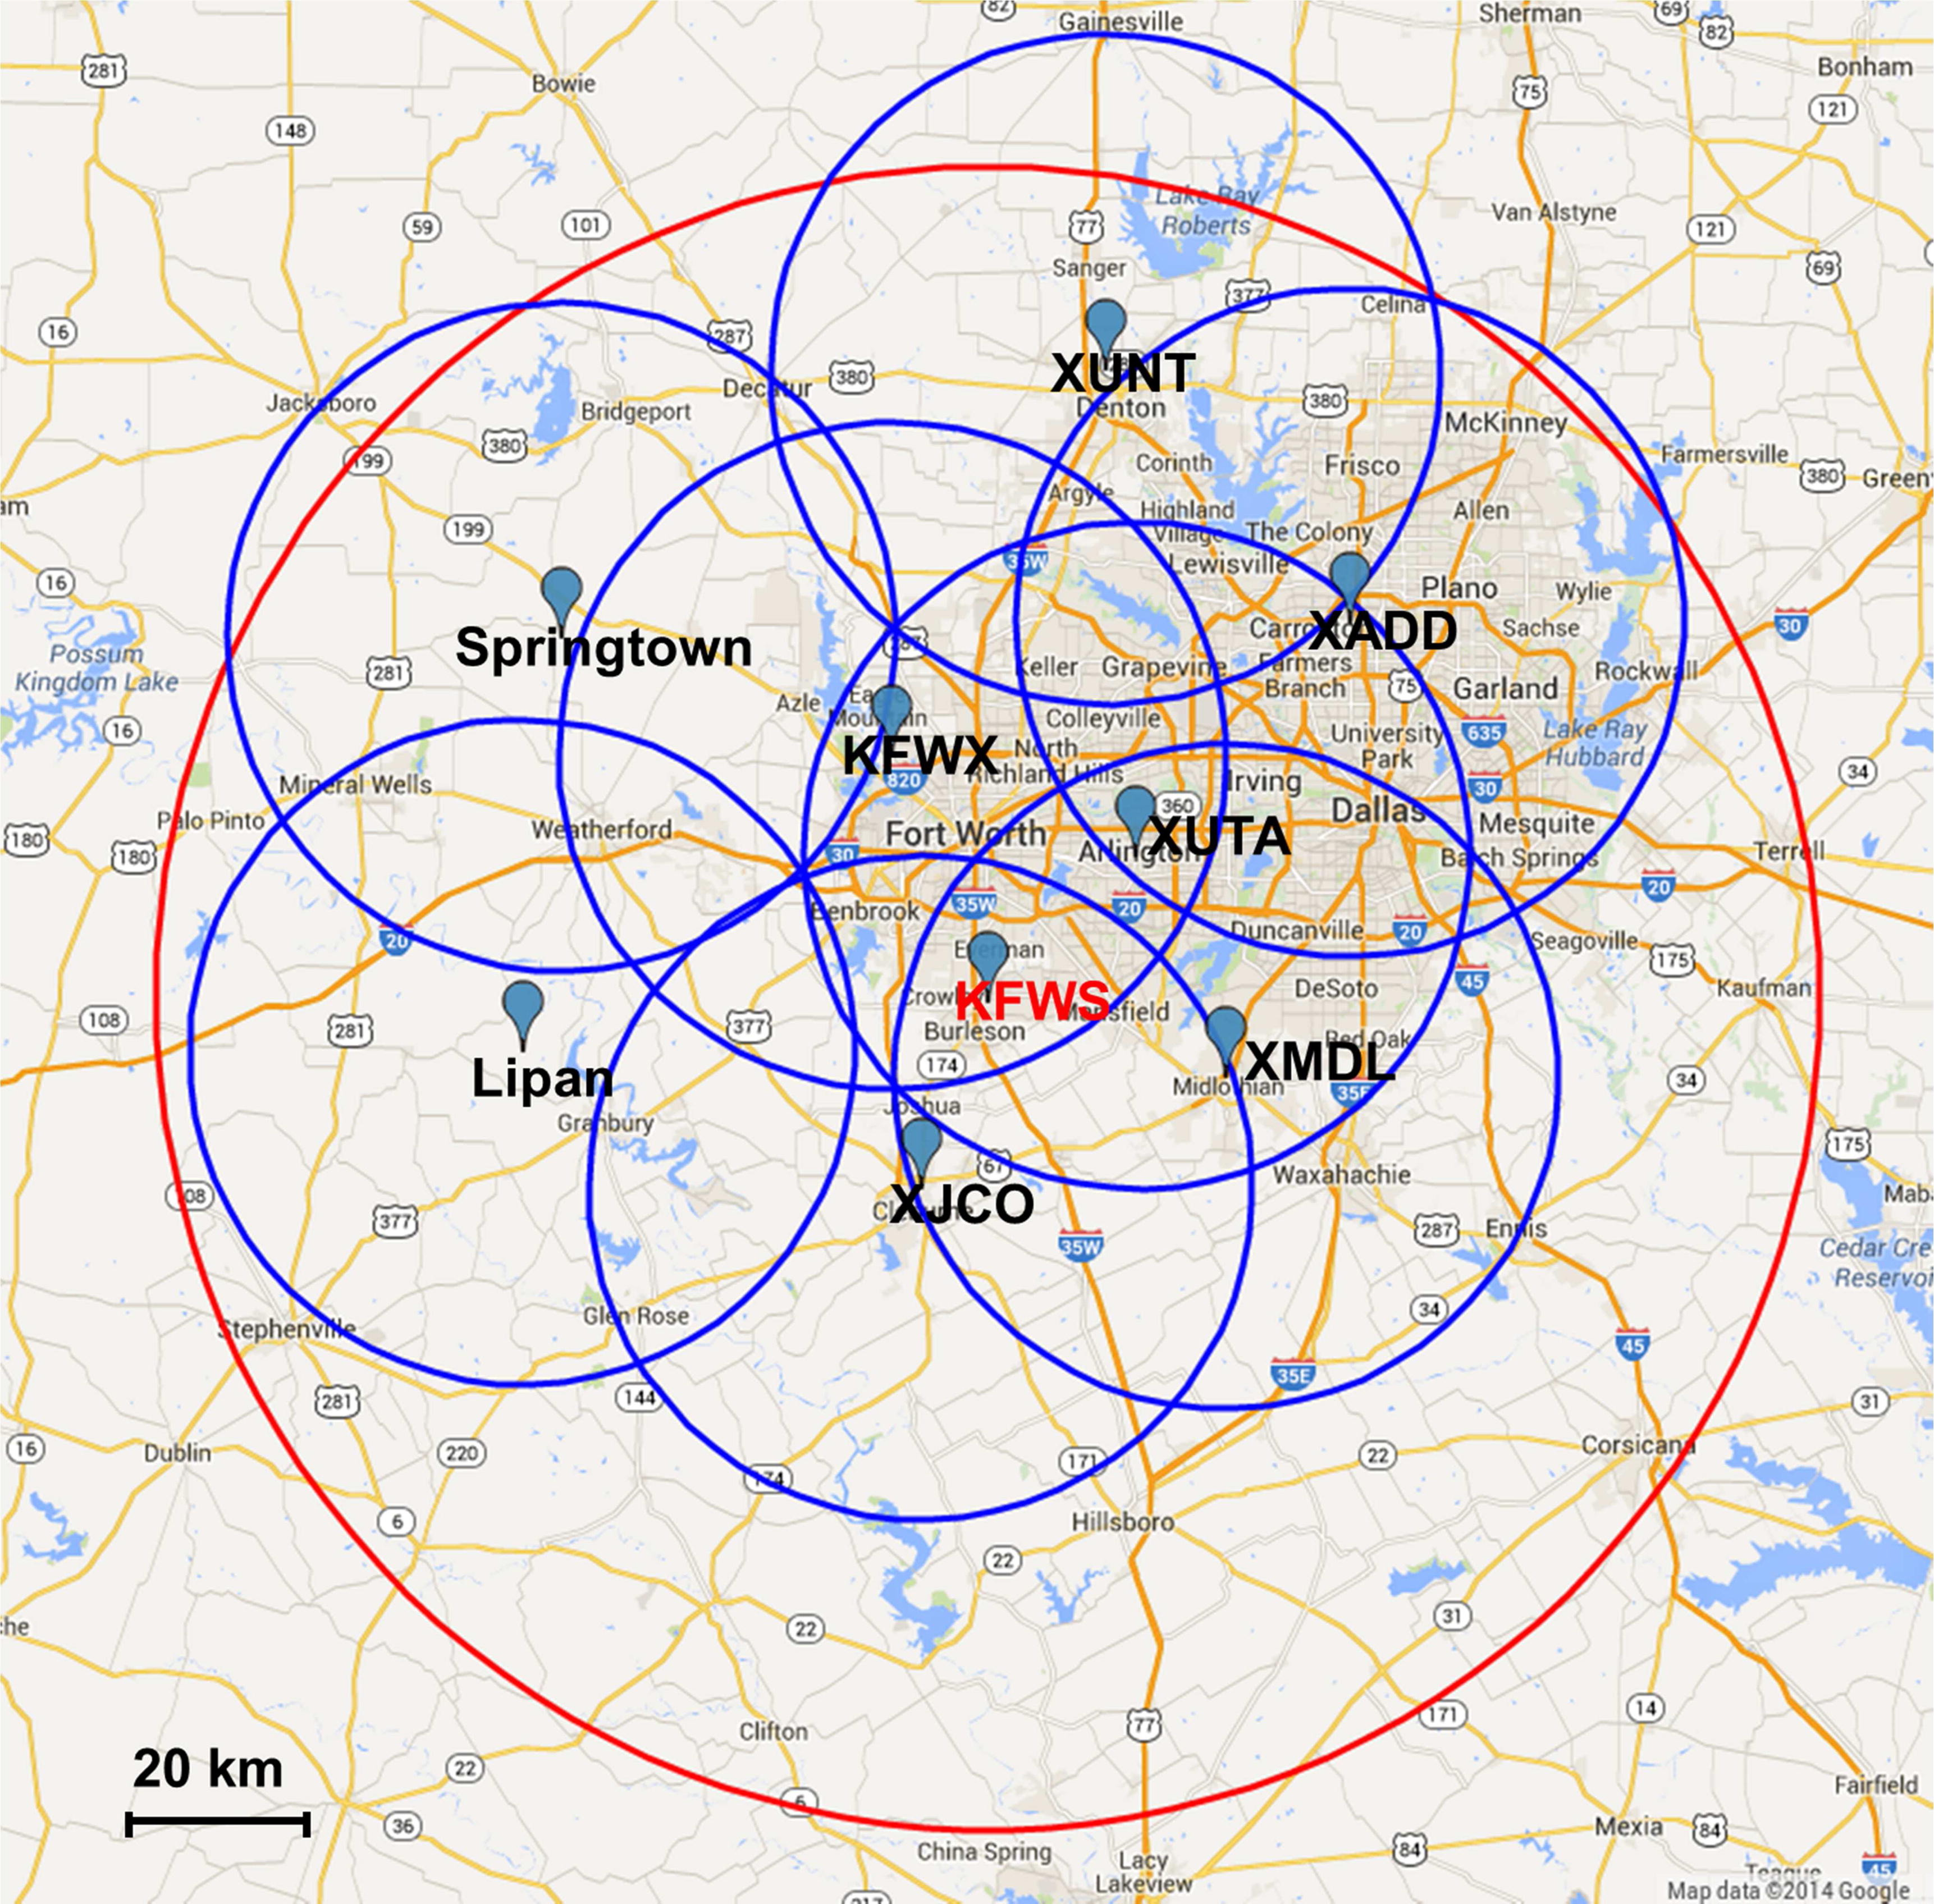
\includegraphics[width=\textwidth]{./thesis_code/plots/casa_dfw_map.jpg}
	\caption{The CASA DFW Urban Testbed network of dual polarimetric X-band Doppler weather radars \cite{chen2015quantitative}, plotted on Google Maps.}
	\label{fig:background_casamap}
\end{figure}

Many of the features and products provided by the CASA DFW system are irrelevant in the present work, including the three-dimensional wind fields and high-resolution rain rate products.
Instead, this research focuses on classifying images produced from single weather radars, and as such can use dual-polarimetric radar variables from each of the radars in the network individually.
Data from each radar in the network are analyzed by signal processing servers at each radar, and the radar variables are stored at the DFW Radar Operations Center (DROC) in two ways: first, all moment data from each completed PPI scan is stored in NetCDF-format files on DROC servers; and second, Portable Network Graphics (PNG) files are generated at each of three elevation scan angles, for each of four radar moments, including horizontal reflectivity, copolar correlation coefficient, differential reflectivity, and radial velocity.

\subsection{NEXRAD}
\label{ssec:background_nexrad}

NEXRAD is a network of WSR-88D S-band radars that are intended to provide weather radar data throughout the United States with minimal gaps in coverage. 
The above concerns regarding Earth curvature, ground clutter, and coverage gaps notwithstanding, the network represented a massive undertaking by the National Weather Service, and serves to this day as a major data provider in the geosciences. 
Recently, the data was moved to be stored in Amazon Web Services cloud storage, further increasing ease of access for recent and historical weather data. 
The data produced from this network is used in weather prediction, as comparison with other sensors, and as inputs to high resolution models for short-, medium-, and long-term forecasting.

When testing these models, atmospheric data scientists are presented with many challenges, including identifying phenomena of interest in the prohibitively voluminous datasets. 
As such, it is of critical importance to develop automated methods for discovering insights and phenomena that are present in the available data, as a way to build datasets and improve forecast model fidelity.
